% Bản tiếng Việt. Biên dịch bằng XeLaTeX (Overleaf: Menu -> Compiler -> XeLaTeX) hoặc `tectonic -X compile main.tex`.
% Bảng và số liệu trong generated/vi/ được sinh bởi make_tables.py từ reports/evidence/.
\documentclass[sigconf,nonacm]{acmart}

\usepackage[vietnamese]{babel}
\usepackage{booktabs}
\usepackage{array}
\usepackage{amsmath}

% Auto-generated by make_tables.py - do not edit
\newcommand{\FZeroAP}{0{,}171}
\newcommand{\FZeroVal}{0{,}064}
\newcommand{\FZeroFone}{0{,}246}
\newcommand{\FZeroPk}{0{,}318}
\newcommand{\FZeroRk}{0{,}177}
\newcommand{\FZeroHits}{318}
\newcommand{\FOneAP}{0{,}534}
\newcommand{\FOneVal}{0{,}477}
\newcommand{\FOneFone}{0{,}534}
\newcommand{\FOnePk}{0{,}712}
\newcommand{\FOneRk}{0{,}396}
\newcommand{\FOneHits}{712}
\newcommand{\FTwoAP}{0{,}662}
\newcommand{\FTwoVal}{0{,}583}
\newcommand{\FTwoFone}{0{,}664}
\newcommand{\FTwoPk}{0{,}893}
\newcommand{\FTwoRk}{0{,}497}
\newcommand{\FTwoHits}{893}
\newcommand{\FThreeAP}{0{,}610}
\newcommand{\FThreeVal}{0{,}521}
\newcommand{\FThreeFone}{0{,}589}
\newcommand{\FThreePk}{0{,}798}
\newcommand{\FThreeRk}{0{,}444}
\newcommand{\FThreeHits}{798}
\newcommand{\FFourAP}{0{,}684}
\newcommand{\FFourVal}{0{,}592}
\newcommand{\FFourFone}{0{,}685}
\newcommand{\FFourPk}{0{,}915}
\newcommand{\FFourRk}{0{,}509}
\newcommand{\FFourHits}{915}
\newcommand{\FFourPkPct}{91{,}50}
\newcommand{\FFourRkPct}{50{,}89}
\newcommand{\FZeroAPpre}{0{,}071}
\newcommand{\FZeroAPpost}{0{,}973}
\newcommand{\FOneAPpre}{0{,}333}
\newcommand{\FOneAPpost}{0{,}962}
\newcommand{\FTwoAPpre}{0{,}506}
\newcommand{\FTwoAPpost}{0{,}958}
\newcommand{\FThreeAPpre}{0{,}413}
\newcommand{\FThreeAPpost}{0{,}962}
\newcommand{\FFourAPpre}{0{,}528}
\newcommand{\FFourAPpost}{0{,}961}
\newcommand{\EZeroAP}{0{,}670}
\newcommand{\EZeroFone}{0{,}673}
\newcommand{\ERAP}{0{,}662}
\newcommand{\ERFone}{0{,}664}
\newcommand{\ERDisc}{0{,}502}
\newcommand{\ERKS}{0{,}019}
\newcommand{\EOneAP}{0{,}673}
\newcommand{\EOneFone}{0{,}674}
\newcommand{\EOneDisc}{0{,}647}
\newcommand{\EOneKS}{0{,}047}
\newcommand{\ETwoAP}{0{,}648}
\newcommand{\ETwoFone}{0{,}625}
\newcommand{\ETwoDisc}{0{,}999}
\newcommand{\ETwoKS}{0{,}221}
\newcommand{\ELLMaAP}{0{,}609}
\newcommand{\ELLMaFone}{0{,}588}
\newcommand{\ELLMaDisc}{0{,}983}
\newcommand{\ELLMaKS}{0{,}126}
\newcommand{\ELLMbAP}{0{,}597}
\newcommand{\ELLMbFone}{0{,}493}
\newcommand{\ELLMbDisc}{0{,}996}
\newcommand{\ELLMbKS}{0{,}139}
\newcommand{\ERDelta}{$-$0{,}0077}
\newcommand{\EOneDelta}{0{,}0026}
\newcommand{\ETwoDelta}{$-$0{,}0221}
\newcommand{\ELLMaDelta}{$-$0{,}0611}
\newcommand{\ELLMbDelta}{$-$0{,}0732}


\providecommand{\keywordsname}{Keywords}
\addto\captionsvietnamese{\renewcommand{\abstractname}{Tóm tắt}\renewcommand{\keywordsname}{Từ khóa}}
\settopmatter{printfolios=true}
\setlength{\emergencystretch}{1.5em}

\begin{document}

\title{Phát hiện rửa tiền bằng machine learning}
\subtitle{Đồ án môn học An toàn và Bảo mật Hệ thống Thông tin}

\author{Nguyễn Thế Vĩnh}
\email{26848266@grad.uit.edu.vn}
\affiliation{%
  \institution{Trường Đại học Công nghệ Thông tin, ĐHQG-HCM}
  \city{TP. Hồ Chí Minh}
  \country{Việt Nam}}

\author{Hoàng Đức Chung}
\email{26848014@grad.uit.edu.vn}
\affiliation{%
  \institution{Trường Đại học Công nghệ Thông tin, ĐHQG-HCM}
  \city{TP. Hồ Chí Minh}
  \country{Việt Nam}}

\author{Nguyễn Hải Đăng}
\email{26848027@grad.uit.edu.vn}
\affiliation{%
  \institution{Trường Đại học Công nghệ Thông tin, ĐHQG-HCM}
  \city{TP. Hồ Chí Minh}
  \country{Việt Nam}}

\renewcommand{\shortauthors}{Nguyễn Thế Vĩnh, Hoàng Đức Chung và Nguyễn Hải Đăng}

\begin{abstract}
Phát hiện giao dịch rửa tiền bằng machine learning gặp hai trở ngại: positive class cực hiếm và tín hiệu nằm ở
bối cảnh hành vi chứ không ở từng giao dịch đơn lẻ. Bài báo so sánh hai hướng cải thiện trong cùng một quy trình
evaluation trên 5.078.345 giao dịch của bộ dữ liệu mô phỏng IBM AML HI-Small: \emph{data augmentation} cho positive
class bằng random oversampling, SMOTENC, CTGAN và Large Language Model (LLM), và \emph{cải thiện biểu diễn} bằng
temporal behavioral feature. Chúng tôi xây dựng 63 feature về lịch sử tài khoản, hoạt động theo time window và quan
hệ đối tác, được tính nghiêm ngặt chỉ từ các giao dịch xảy ra trước thời điểm dự đoán, và giữ cố định classifier
XGBoost. Bổ sung lần lượt các feature group nâng Average Precision (AP) từ \FZeroAP{} lên \FOneAP{} và \FFourAP;
với alert budget 1.000 alert có score cao nhất, cấu hình đầy đủ đạt precision \FFourPkPct\% và recall
\FFourRkPct\%. Ngược lại, không phương pháp data augmentation nào cải thiện rõ rệt so với không augmentation; hai
biến thể LLM giảm AP từ \EZeroAP{} xuống \ELLMaAP{} và \ELLMbAP, và synthetic data do CTGAN hoặc LLM sinh ra gần
như bị phân biệt hoàn toàn với dữ liệu thật (discriminator AUC $\geq$ \ELLMaDisc). Phân tích bổ sung phát hiện
distribution shift mạnh từ ngày 11/09/2022; trên phần test trước mốc này, lợi ích của behavioral feature vẫn được
duy trì. Kết quả cho thấy với dữ liệu giao dịch, chất lượng feature engineering và tính đúng đắn theo thời gian
của pipeline quan trọng hơn việc bổ sung synthetic data.
\end{abstract}

\keywords{anti-money laundering, transaction monitoring, XGBoost, temporal feature, feature engineering,
data augmentation, Large Language Model, data leakage}

\maketitle
\pagestyle{plain}  % no running head (title/authors) on later pages, page number only

% ======================================================================
\section{Giới thiệu}

Rửa tiền (money laundering) là quá trình hợp thức hóa nguồn tiền bất hợp pháp thông qua chuỗi giao dịch nhằm che
giấu nguồn gốc. Các tổ chức tài chính có nghĩa vụ transaction monitoring và báo cáo giao dịch đáng ngờ theo khuyến
nghị của FATF~\cite{fatf2012} và, tại Việt Nam, theo Luật Phòng, chống rửa tiền 2022~\cite{luatpcrt2022}. Dưới góc
nhìn an toàn hệ thống thông tin, hệ thống transaction monitoring đóng vai trò tương tự một intrusion detection system:
nó phải xếp hạng một luồng sự kiện rất lớn, trong đó chỉ một tỷ lệ nhỏ là độc hại, và mỗi false positive đều tiêu
tốn thời gian của chuyên viên điều tra.

Phát hiện rửa tiền bằng machine learning gặp ba khó khăn. Thứ nhất, positive class cực hiếm: trong bộ dữ liệu IBM
AML HI-Small~\cite{altman2023realistic} chỉ khoảng 0,1\% giao dịch được gán nhãn rửa tiền (class imbalance). Thứ hai,
một giao dịch đơn lẻ hầu như không mang tín hiệu; dấu hiệu nằm ở \emph{bối cảnh} như lịch sử tài khoản, nhịp độ
giao dịch và mối quan hệ giữa các tài khoản. Thứ ba, dữ liệu có thứ tự thời gian, nên rất dễ vô tình để model ``nhìn
thấy tương lai'' khi feature engineering (temporal leakage), dẫn tới kết quả lạc quan giả tạo.

Có hai hướng phổ biến để cải thiện detector. Hướng thứ nhất là \emph{data augmentation} cho positive class bằng
oversampling, SMOTE~\cite{chawla2002smote}, generative model như CTGAN~\cite{xu2019ctgan}, hoặc gần đây là
LLM~\cite{borisov2023great,seedat2024cllm}. Hướng thứ hai là \emph{feature engineering}: mô tả hành vi theo thời gian
của tài khoản và quan hệ giữa các tài khoản~\cite{blanusa2024gfp,deprez2024network}. Bài báo này so sánh hai hướng
trên trong cùng một quy trình: cùng temporal split, cùng classifier XGBoost~\cite{chen2016xgboost} với hyperparameter
cố định, cùng cách chọn threshold trên validation set và ba seed. Các đóng góp chính gồm:

\begin{itemize}
  \item Một feature set gồm 63 behavioral feature được tính \emph{nghiêm ngặt theo thời gian}: chỉ dùng giao dịch có
  thời điểm nhỏ hơn thời điểm dự đoán, các giao dịch cùng phút dùng chung một snapshot lịch sử, và các tổng tiền được
  tách theo currency.
  \item Một ablation study có kiểm soát gồm năm cấu hình định trước, cho thấy AP tăng từ \FZeroAP{} lên \FFourAP{} và
  mọi bước bổ sung đều cải thiện AP trong cả ba seed.
  \item Evaluation bốn phương pháp data augmentation, gồm hai biến thể sinh dữ liệu bằng LLM, kèm chẩn đoán chất lượng
  synthetic data. Không phương pháp nào cải thiện rõ rệt; synthetic data của CTGAN và LLM gần như bị tách biệt hoàn
  toàn khỏi dữ liệu thật.
  \item Phân tích tính hợp lệ của evaluation: time policy, distribution shift từ ngày 11/09/2022 và việc tái sử dụng
  test set, cùng quy trình xác minh kết quả có thể tái lập (reproducible).
\end{itemize}

% ======================================================================
\section{Công trình liên quan}

\paragraph{Dataset và benchmark} Do dữ liệu ngân hàng thật không thể công bố, nghiên cứu học thuật chủ yếu dùng dữ
liệu công khai như transaction graph Bitcoin Elliptic~\cite{weber2019elliptic} hoặc dữ liệu mô phỏng. Altman và cộng
sự~\cite{altman2023realistic} công bố trình sinh AMLworld dựa trên agent-based simulation và sáu dataset giao dịch
ngân hàng tổng hợp có nhãn đầy đủ~\cite{ibmamlkaggle}; HI-Small là dataset nhỏ nhất với tỷ lệ giao dịch rửa tiền
cao hơn (HI: higher illicit ratio).

\paragraph{Graph feature và GNN} Graph Feature Preprocessor (GFP)~\cite{blanusa2024gfp}, thuộc thư viện Snap
ML~\cite{dunner2018snapml}, trích xuất theo thời gian thực các pattern fan-in/fan-out, scatter-gather và cycle, cùng
vertex statistics trong time window, rồi đưa vào gradient boosting model; trên HI-Small cách làm này đạt minority-class
F1 khoảng 0,63--0,65 và vượt các Graph Neural Network (GNN) tiêu chuẩn. Multi-GNN~\cite{egressy2024multignn} mở rộng
GNN cho directed multigraph. Deprez và cộng sự~\cite{deprez2024network} tổng quan 97 công trình và cho thấy thông tin
network cải thiện khả năng dự đoán. Các công trình gần đây tập trung vào tốc độ pattern mining~\cite{ye2026blazingaml}
hoặc biểu diễn quasi-temporal graph~\cite{tariq2026exstraqt}. Ngược lại, Effendi và Chattopadhyay~\cite{effendi2024fhe}
ghi nhận XGBoost có thể không cần graph feature trong một số cấu hình dữ liệu. Bài báo này không tái hiện GFP mà tập
trung vào các thống kê hành vi và quan hệ cục bộ có thể giải thích trực tiếp.

\paragraph{Data augmentation và LLM} SMOTE~\cite{chawla2002smote} nội suy giữa các minority sample;
CTGAN~\cite{xu2019ctgan} học phân phối tabular data bằng conditional GAN. LLM được dùng để sinh tabular
data~\cite{borisov2023great}, kết hợp với data curation trong low-data regime~\cite{seedat2024cllm}, hoặc để tự động
đề xuất feature~\cite{hollmann2023caafe,abhyankar2025llmfe}. Chúng tôi đánh giá khả năng sinh giao dịch rửa tiền bằng
LLM trong feature space cho bài toán cực kỳ mất cân bằng.

% ======================================================================
\section{Dữ liệu và bài toán}

\paragraph{Dataset} Chúng tôi dùng tệp \texttt{HI-Small\_Trans.csv} của IBM AML~\cite{ibmamlkaggle} gồm 5.078.345
giao dịch trong khoảng 01--18/09/2022, trong đó 5.177 giao dịch (0,102\%) được gán nhãn rửa tiền. Mỗi giao dịch có
timestamp (độ phân giải phút), ngân hàng và tài khoản của sender/receiver, số tiền và currency hai phía, payment format
và nhãn. Tệp được đối chiếu bằng SHA-256 hash giữa môi trường cục bộ và Kaggle. Tài khoản được định danh bằng cặp
ngân hàng--mã tài khoản; định danh chỉ dùng để tra cứu lịch sử, không đưa vào model.

\paragraph{Bài toán} Mỗi giao dịch là một sample. Model trả về suspicion score để xếp hạng; quyết định nhị phân dùng
threshold chọn trên validation set. Score không được calibrate thành xác suất rủi ro.

\paragraph{Temporal split} Dữ liệu được sắp xếp theo timestamp và chia xấp xỉ 60/20/20; điểm cắt được dịch về đầu
nhóm giao dịch cùng phút để một phút không bị tách sang hai tập (Bảng~\ref{tab:split}). Không shuffle dữ liệu; nhãn
của validation và test set không tham gia feature engineering hay training.

\begin{table}[t]
\caption{Temporal split của dữ liệu.}
\label{tab:split}
\small
\setlength{\tabcolsep}{4pt}
\begin{tabular}{lrrrl}
\toprule
Tập & Giao dịch & Positive & Tỷ lệ & Khoảng thời gian \\
\midrule
Train & 3.046.861 & 2.297 & 0,075\% & 01/09 -- 06/09 13:35 \\
Validation & 1.015.602 & 1.082 & 0,107\% & 06/09 13:36 -- 08/09 16:11 \\
Test & 1.015.882 & 1.798 & 0,177\% & 08/09 16:12 -- 18/09 \\
\bottomrule
\end{tabular}
\end{table}

% ======================================================================
\section{Phương pháp}

\subsection{Time policy}

Gọi $t$ là timestamp của giao dịch cần dự đoán. Tập lịch sử được phép quan sát là
\begin{equation}
H(t) = \{\, j : t_j < t \,\}.
\end{equation}
Vì dữ liệu chỉ chính xác đến phút và thứ tự thật trong cùng phút là không biết, mọi giao dịch cùng timestamp dùng chung
một snapshot lịch sử; lịch sử chỉ được cập nhật sau khi cả nhóm đã được truy vấn. Nhờ vậy feature không phụ thuộc thứ
tự dòng trong tệp. Self-transfer tạo một sự kiện gửi và một sự kiện nhận, và sự kiện gửi của chính giao dịch không trở
thành lịch sử của phía nhận. Time window độ dài $W$ được định nghĩa là $[t-W, t)$. Các giao dịch không nhãn đã xảy
ra trong validation và test set được phép bổ sung lịch sử cho giao dịch đến sau, tương ứng với việc quan sát luồng
giao dịch theo thời gian.

\subsection{Behavioral feature}

Feature set gồm bốn feature group, tổng cộng 63 cột:
\begin{itemize}
  \item \textbf{Transaction (11):} log số tiền gửi/nhận, giờ, thứ, payment format, currency hai phía, cùng ngân hàng,
  self-transfer, đổi currency, số tiền tròn trăm.
  \item \textbf{History (17):} với mỗi tài khoản sender và receiver: số giao dịch trước đó, số lượt gửi và nhận, trung
  bình log số tiền gửi và nhận, thời gian từ giao dịch gần nhất, số giao dịch cùng ngày tổng và theo hướng; thêm số
  giao dịch trước đó của cặp sender$\to$receiver.
  \item \textbf{Activity (20):} với time window 1 giờ và 24 giờ, số lượt và log tổng tiền theo hướng của mỗi tài
  khoản, cùng độ lệch giữa log số tiền hiện tại và trung bình log lịch sử cùng hướng. Các tổng tiền và độ lệch được
  tính riêng theo tài khoản \emph{và currency}, không cộng các currency khác nhau khi không có tỷ giá. Sliding sum dùng
  Neumaier compensated summation để không để lại sai số khi các khoản tiền chênh lệch rất lớn rời khỏi window.
  \item \textbf{Relationship (15):} số counterparty duy nhất theo hướng và window, số giao dịch lịch sử của cặp đảo
  chiều, tuổi và độ gần (recency) của quan hệ sender$\to$receiver, số giao dịch của cặp trong window, và counterparty
  share trong 24 giờ (số giao dịch A$\to$B chia số lượt gửi của A).
\end{itemize}
Khi không có lịch sử, số đếm và tổng bằng 0, còn trung bình và khoảng thời gian để NaN cho XGBoost tự xử lý. Năm cấu
hình được xác định trước khi chạy: F0 = Transaction; F1 = F0 + History; F2 = F1 + Activity; F3 = F1 + Relationship;
F4 = F1 + Activity + Relationship. Hiệu số F1$-$F0 đo tác động của History; F2$-$F1 và F3$-$F1 đo lợi ích của từng
group khi đã có History; F4$-$F2 và F4$-$F3 đo phần bổ sung của group còn lại. Feature được tính bằng các linear scan
theo tài khoản, tăng tốc bằng Numba.

\subsection{Data augmentation}

Các phương pháp augmentation chỉ bổ sung giao dịch rửa tiền tổng hợp vào train set; validation và test set luôn là dữ
liệu thật. Số synthetic sample bằng 0,5 lần số positive sample của train set (1.148 sample mỗi lượt). Chúng tôi so
sánh: \textbf{ER} random oversampling positive sample; \textbf{E1} SMOTENC trên feature đã chuẩn hóa, categorical
feature lấy mode của các nearest neighbor; \textbf{E2} CTGAN 300 epoch chỉ học trên positive sample; \textbf{E3a/E3b}
một LLM thương mại qua OpenAI API sinh giao dịch rửa tiền dạng JSON từ các example thật, thống kê cột và các ràng buộc
logic giữa các cột, trong đó E3b bổ sung mô tả các laundering typology của AMLworld vào prompt. Output của LLM được
validate, loại duplicate và loại các dòng sao chép nguyên văn dữ liệu thật; chi phí API được giới hạn bằng một budget
ledger. Chất lượng synthetic data được đo bằng thống kê Kolmogorov--Smirnov (KS) trung bình theo cột so với positive
sample thật, và bằng AUC của một XGBoost discriminator phân biệt thật/giả (\emph{discriminator AUC}; 0,5 nghĩa là
không phân biệt được).

Thí nghiệm augmentation được thực hiện trước feature study, trên pipeline 28 feature tương ứng F1 nhưng xử lý các
giao dịch cùng phút theo thứ tự dòng ổn định trong tệp. Vì khác protocol, chúng tôi chỉ so sánh các phương pháp
augmentation với nhau, không so sánh con số tuyệt đối với F0--F4.

\subsection{Model và evaluation}

Mọi cấu hình dùng XGBoost với tối đa 1.000 cây, learning rate 0,05, max depth 8, subsample và colsample\_bytree 0,8,
min child weight 1, \texttt{hist} tree method trên GPU, early stopping sau 100 vòng theo AUC-PR trên validation set.
Không có hyperparameter tuning riêng cho từng cấu hình và không resampling tỷ lệ lớp. Threshold tối đa F1 được chọn
trên validation set của từng lượt chạy rồi áp dụng nguyên cho test set.

Metric chính là Average Precision (AP), tính bằng hàm average precision của scikit-learn. Ngoài ra chúng tôi báo cáo
F1 tại threshold và Precision@1000/Recall@1000: tỷ lệ giao dịch rửa tiền trong 1.000 alert có score cao nhất trên
toàn test set, và tỷ lệ giao dịch rửa tiền của test set nằm trong danh sách đó. Accuracy không được dùng vì positive
class rất hiếm. Mỗi cấu hình chạy ba seed (0, 1, 2); bảng trình bày mean $\pm$ sample standard deviation (SD), và các
so sánh dùng paired difference theo cùng seed. SD này phản ánh biến động training trên cùng test set, không phải
confidence interval trên quần thể giao dịch mới.

\subsection{Verification và reproducibility}

Pipeline có 43 regression test: biên thời gian và window, self-transfer, currency, tính bất biến khi đổi thứ tự các
dòng cùng timestamp, tính độc lập với nhãn và tương lai, và đối chiếu với cách tính trực tiếp trên mẫu nhỏ. Sau khi
chạy, 30 prediction file của 15 lượt được kiểm tra lại về nhãn, thứ tự, AP, metric tại threshold và việc threshold
được chọn trên validation set. Một manifest ghi hash của dữ liệu và source code, phiên bản thư viện, danh sách cột và
thông tin split. Các lượt chạy được thực hiện trên Kaggle notebook riêng tư với hai GPU Tesla T4, NumPy 2.2.6, pandas
2.3.3, scikit-learn 1.7.2, XGBoost 3.1.1 và Numba 0.61.2.

% ======================================================================
\section{Kết quả thực nghiệm}

\subsection{Ablation study theo feature group}

\begin{table*}[t]
\caption{Ablation study theo feature group (mean $\pm$ SD qua ba seed). AP được báo cáo trên test và validation set;
các metric còn lại trên test set.}
\label{tab:features}
\begin{tabular}{lrccccc}
\toprule
Cấu hình & Số feature & AP (test) & AP (validation) & F1 & Precision@1000 & Recall@1000 \\
\midrule
F0 Transaction & 11 & 0{,}171 $\pm$ 0{,}002 & 0{,}064 $\pm$ 0{,}001 & 0{,}246 $\pm$ 0{,}016 & 0{,}318 $\pm$ 0{,}007 & 0{,}177 $\pm$ 0{,}004 \\
F1 +History & 28 & 0{,}534 $\pm$ 0{,}037 & 0{,}477 $\pm$ 0{,}026 & 0{,}534 $\pm$ 0{,}028 & 0{,}712 $\pm$ 0{,}033 & 0{,}396 $\pm$ 0{,}018 \\
F2 +Activity & 48 & 0{,}662 $\pm$ 0{,}020 & 0{,}583 $\pm$ 0{,}014 & 0{,}664 $\pm$ 0{,}016 & 0{,}893 $\pm$ 0{,}013 & 0{,}497 $\pm$ 0{,}007 \\
F3 +Relationship & 43 & 0{,}610 $\pm$ 0{,}014 & 0{,}521 $\pm$ 0{,}026 & 0{,}589 $\pm$ 0{,}026 & 0{,}798 $\pm$ 0{,}016 & 0{,}444 $\pm$ 0{,}009 \\
F4 Combined & 63 & \textbf{0{,}684 $\pm$ 0{,}025} & \textbf{0{,}592 $\pm$ 0{,}023} & \textbf{0{,}685 $\pm$ 0{,}026} & \textbf{0{,}915 $\pm$ 0{,}013} & \textbf{0{,}509 $\pm$ 0{,}007} \\
\bottomrule

\end{tabular}
\end{table*}

Bảng~\ref{tab:features} cho thấy chỉ dùng thuộc tính của từng giao dịch (F0) cho AP \FZeroAP. Bổ sung History (F1)
tạo bước nhảy lớn nhất, lên \FOneAP. Khi đã có History, Activity group (F2, \FTwoAP) đóng góp nhiều hơn Relationship
group (F3, \FThreeAP), và kết hợp cả hai (F4) đạt AP cao nhất, \FFourAP. Thứ tự các cấu hình giống nhau trên
validation và test set. Bảng~\ref{tab:fsdelta} cho thấy mọi bước bổ sung đều cải thiện AP trong cả ba seed, kể cả F4
so với F2: Relationship group vẫn mang thông tin bổ sung khi đã có Activity group. Ba seed chỉ đủ mô tả tính nhất
quán của các lượt chạy này, chưa đủ để khẳng định statistical significance.

\begin{table}[t]
\caption{Paired difference của AP trên test set theo cùng seed.}
\label{tab:fsdelta}
\small
\begin{tabular}{lccc}
\toprule
So sánh & Mean $\Delta$AP & SD & Số seed tăng \\
\midrule
F1 $-$ F0 & +0{,}3631 & 0{,}0371 & 3/3 \\
F2 $-$ F1 & +0{,}1278 & 0{,}0165 & 3/3 \\
F3 $-$ F1 & +0{,}0765 & 0{,}0233 & 3/3 \\
F4 $-$ F1 & +0{,}1502 & 0{,}0122 & 3/3 \\
F4 $-$ F2 & +0{,}0224 & 0{,}0043 & 3/3 \\
F4 $-$ F3 & +0{,}0737 & 0{,}0112 & 3/3 \\
\bottomrule

\end{tabular}
\end{table}

\begin{figure}[t]
\centering
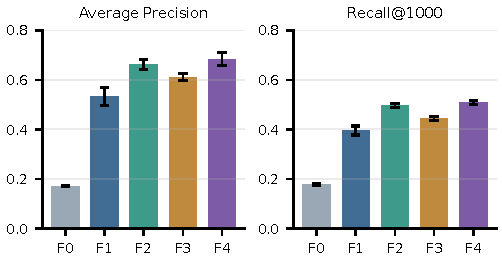
\includegraphics[width=\linewidth]{figures/feature_ablation.pdf}
\caption{AP và Recall@1000 của năm cấu hình feature; error bar là SD qua ba seed trên cùng test set.}
\label{fig:ablation}
\end{figure}

\subsection{Ý nghĩa theo alert budget}

Test set có 1.798 giao dịch rửa tiền. Trong 1.000 alert có score cao nhất, F1 tìm được trung bình khoảng \FOneHits{}
giao dịch rửa tiền, còn F4 tìm được \FFourHits; số false positive giảm tương ứng trong khi khối lượng công việc của
chuyên viên vẫn là 1.000 alert. Tuy vậy, recall \FFourRk{} cũng có nghĩa là gần một nửa số giao dịch rửa tiền nằm
ngoài danh sách. Alert budget 1.000 alert cho toàn test set là một giả định thực nghiệm; hệ thống thật có thể cần
giới hạn theo ngày hoặc theo năng lực xử lý của bộ phận điều tra.

\subsection{Feature importance}

\begin{table}[t]
\caption{Mười feature có tỷ trọng total gain trung bình cao nhất trong F4 (ba seed).}
\label{tab:importance}
\small
\begin{tabular}{r>{\raggedright\arraybackslash}p{4.1cm}lr}
\toprule
\# & Feature & Group & Gain (\%) \\
\midrule
1 & Số lượt nhận trước đó của sender & History & 7{,}74 \\
2 & Thời gian từ giao dịch gần nhất của receiver & History & 7{,}05 \\
3 & Độ lệch số tiền so với lịch sử gửi (cùng currency) & Activity & 6{,}35 \\
4 & Payment format & Transaction & 5{,}27 \\
5 & Giờ trong ngày & Transaction & 4{,}77 \\
6 & Số giao dịch trước đó của cặp sender$\to$receiver & History & 4{,}64 \\
7 & Độ lệch số tiền so với lịch sử nhận của sender & Activity & 4{,}29 \\
8 & Độ lệch số tiền so với lịch sử nhận của receiver & Activity & 3{,}71 \\
9 & Log tổng tiền sender đã nhận trong 24 giờ & Activity & 3{,}70 \\
10 & Trung bình log số tiền sender đã nhận & History & 3{,}51 \\
\bottomrule

\end{tabular}
\end{table}

Bảng~\ref{tab:importance} cho thấy các feature quan trọng nhất kết hợp thuộc tính hiện tại với bối cảnh tài khoản: số
lượt nhận trước đó của sender, thời gian từ giao dịch gần nhất của receiver, độ lệch số tiền so với lịch sử cùng
currency, payment format và số lần cặp tài khoản đã giao dịch. Điều này phù hợp với trực giác nghiệp vụ: tài khoản vừa
nhận tiền rồi chuyển đi với số tiền bất thường so với thói quen là dấu hiệu của money mule. Tuy nhiên, gain importance
của cây bị ảnh hưởng bởi tương quan giữa các cột, nên không được diễn giải như tác động nhân quả và không thay thế
ablation study theo group ở trên.

\subsection{Data augmentation}

\begin{table*}[t]
\caption{Data augmentation cho train set (protocol của pipeline trước, 28 feature; ba seed). KS và discriminator AUC
đo khoảng cách giữa synthetic sample và positive sample thật; discriminator AUC càng gần 0,5 thì synthetic data càng
giống thật.}
\label{tab:aug}
\begin{tabular}{lccccc}
\toprule
Phương pháp & AP & F1 & Precision@1000 & Mean KS & Discriminator AUC \\
\midrule
E0 No augmentation & 0{,}670 $\pm$ 0{,}008 & 0{,}673 $\pm$ 0{,}010 & 0{,}902 & -- & -- \\
ER Random oversampling & 0{,}662 $\pm$ 0{,}010 & 0{,}664 $\pm$ 0{,}003 & 0{,}894 & 0{,}019 & 0{,}502 \\
E1 SMOTENC & 0{,}673 $\pm$ 0{,}014 & 0{,}674 $\pm$ 0{,}009 & 0{,}899 & 0{,}047 & 0{,}647 \\
E2 CTGAN & 0{,}648 $\pm$ 0{,}014 & 0{,}625 $\pm$ 0{,}016 & 0{,}883 & 0{,}221 & 0{,}999 \\
E3a LLM, basic prompt & 0{,}609 $\pm$ 0{,}015 & 0{,}588 $\pm$ 0{,}018 & 0{,}854 & 0{,}126 & 0{,}983 \\
E3b LLM, AML-aware prompt & 0{,}597 $\pm$ 0{,}051 & 0{,}493 $\pm$ 0{,}181 & 0{,}838 & 0{,}139 & 0{,}996 \\
\bottomrule

\end{tabular}
\end{table*}

Bảng~\ref{tab:aug} cho thấy không phương pháp augmentation nào cải thiện rõ rệt so với không augmentation (AP
\EZeroAP). SMOTENC cho AP \EOneAP, paired difference theo cùng seed chỉ \EOneDelta{} và nằm trong biến động giữa các
seed. Random oversampling giảm nhẹ ($\Delta$AP = \ERDelta), CTGAN giảm \ETwoDelta, còn hai biến thể LLM giảm mạnh
nhất (\ELLMaDelta{} và \ELLMbDelta).

Cột discriminator AUC giải thích hiện tượng này. Sample lặp lại không phân biệt được với sample thật (\ERDisc),
SMOTENC ở mức \EOneDisc, trong khi CTGAN (\ETwoDisc) và LLM (\ELLMaDisc{} và \ELLMbDisc) gần như bị tách biệt hoàn
toàn. Synthetic sample vẫn mang nhãn positive, nên model học thêm những vùng không tồn tại trong dữ liệu thật. Với LLM,
precision tại threshold tăng nhưng recall giảm mạnh: model trở nên ``thận trọng'' hơn và bỏ sót nhiều giao dịch rửa
tiền hơn. Đáng chú ý, bổ sung domain knowledge về các laundering typology vào prompt (E3b) không cải thiện mà còn làm
kết quả kém ổn định hơn giữa các seed (SD của F1 lớn). Với dữ liệu giao dịch, mỗi giao dịch rửa tiền là một phần của
chuỗi có cấu trúc thời gian và quan hệ; sinh từng dòng độc lập trong feature space khó tái tạo được các ràng buộc này.
Đây là lý do thực tế để chúng tôi chuyển trọng tâm sang feature engineering.

\subsection{Distribution shift theo thời gian}

Thống kê theo ngày cho thấy từ 11/09/2022, lưu lượng giao dịch giảm mạnh trong khi tỷ lệ positive label tăng vọt
(Hình~\ref{fig:daily}): ngày 10/09 có 208.325 giao dịch và 442 positive label, ngày 11/09 chỉ có 396 giao dịch nhưng
232 positive label. Trong test set, phần trước 11/09 có 1.014.774 giao dịch với 1.143 positive label (0,113\%), còn
phần từ 11/09 chỉ có 1.108 giao dịch nhưng 655 positive label (59,1\%). Nguyên nhân chưa được xác minh từ cơ chế sinh
dữ liệu. Đây là phát hiện post-hoc, nên chúng tôi không loại phần này khỏi evaluation chính và không training lại, mà
tách các prediction cố định thành hai phần để chẩn đoán (Bảng~\ref{tab:temporal}).

\begin{table}[t]
\caption{AP trên hai phần của test set, tách tại 11/09/2022 (post-hoc diagnostic, cùng các model).}
\label{tab:temporal}
\small
\begin{tabular}{lcc}
\toprule
Cấu hình & Trước 11/09 & Từ 11/09 \\
\midrule
F0 & 0{,}071 $\pm$ 0{,}000 & 0{,}973 $\pm$ 0{,}000 \\
F1 & 0{,}333 $\pm$ 0{,}042 & 0{,}962 $\pm$ 0{,}004 \\
F2 & 0{,}506 $\pm$ 0{,}022 & 0{,}958 $\pm$ 0{,}005 \\
F3 & 0{,}413 $\pm$ 0{,}022 & 0{,}962 $\pm$ 0{,}004 \\
F4 & 0{,}528 $\pm$ 0{,}028 & 0{,}961 $\pm$ 0{,}005 \\
\bottomrule

\end{tabular}
\end{table}

\begin{figure}[t]
\centering
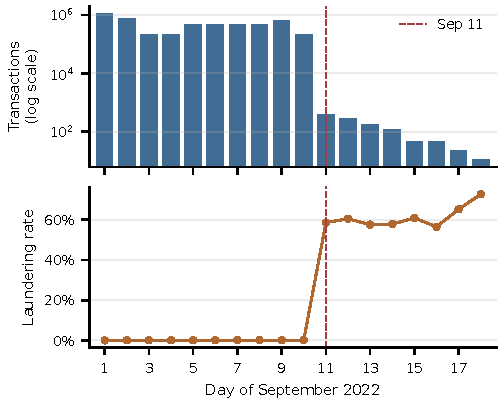
\includegraphics[width=\linewidth]{figures/daily_profile.pdf}
\caption{Số giao dịch (log scale) và tỷ lệ positive label theo ngày trong HI-Small; đường đứt nét đánh dấu 11/09.}
\label{fig:daily}
\end{figure}

Trên phần trước 11/09, F4 vẫn vượt F1 (AP \FFourAPpre{} so với \FOneAPpre), nên lợi ích của feature không chỉ đến từ
phần cuối bất thường. Ở phần cuối, chỉ Transaction feature (F0) đã đạt AP \FZeroAPpost{} và F4 không vượt F0. Vì AP
phụ thuộc tỷ lệ nhãn, chúng tôi chỉ so sánh các cấu hình trong cùng một phần, không so sánh AP giữa hai phần để kết
luận phần nào dễ hơn.

\subsection{Chi phí tính toán}

Trên Kaggle, tạo toàn bộ feature table (gồm đọc dữ liệu và biên dịch JIT) mất khoảng 35,0 giây và feature table
chiếm khoảng 1,33 GB. Training 15 model mất 620,2 giây; toàn bộ lượt chạy, gồm evaluation và ghi tệp, mất 733,3
giây. Các con số mô tả một lượt chạy trên một môi trường cụ thể; chúng tôi chưa đo latency cập nhật feature theo từng
giao dịch trong một online service.

% ======================================================================
\section{Thảo luận}

\paragraph{Ý nghĩa đối với an toàn hệ thống thông tin} Hệ thống transaction monitoring là một thành phần phòng thủ;
chất lượng của nó được đo bằng số giao dịch rửa tiền tìm được trong alert budget mà bộ phận điều tra xử lý được. Kết
quả cho thấy feature engineering quyết định hiệu quả nhiều hơn việc bổ sung synthetic data, và behavioral feature còn
có lợi thế giải thích được (explainable) bằng ngôn ngữ nghiệp vụ, điều cần thiết khi alert phải được chuyên viên xem
xét. Mặt khác, một biểu diễn dựa trên hành vi cũng tạo ra attack surface: kẻ rửa tiền có thể chủ động chia nhỏ giao
dịch (structuring), giãn thời gian hoặc thêm money mule để làm sai lệch các thống kê theo window và quan hệ (evasion
attack). Trong triển khai, hệ thống còn cần access control cho dữ liệu, bảo vệ API key và kết quả alert; source code
công bố của chúng tôi không chứa API key, dữ liệu thô hay prediction của từng giao dịch.

\paragraph{Temporal leakage là một lỗ hổng phương pháp} Một score cao mất ý nghĩa nếu feature dùng thông tin tương
lai, nhãn của tập evaluation, hoặc phụ thuộc vào thứ tự dòng tùy ý của tệp. Pipeline augmentation trước dùng 28
feature tương ứng F1 nhưng xử lý giao dịch cùng phút theo thứ tự dòng, và đạt AP \EZeroAP{} khi không augmentation;
F1 với time policy nghiêm ngặt chỉ đạt \FOneAP. Hai pipeline còn khác nhau ở một số chi tiết cài đặt, nên đây không
phải phép so sánh có kiểm soát. Tuy nhiên, khoảng cách lớn này gợi ý rằng thông tin về các giao dịch cùng phút và thứ
tự của chúng trong tệp có thể làm score tăng đáng kể. Vì vậy, khi so sánh các feature set hoặc so sánh với công trình
khác, time policy phải được cố định và công bố rõ, giống như việc cố định model và temporal split. Cũng vì lý do này,
F1 của F4 (\FFourFone) không nên được so sánh trực tiếp với các con số đã công bố trên HI-Small~\cite{blanusa2024gfp,
egressy2024multignn}: các công trình đó dùng điểm cắt train/test khác (ví dụ Multi-GNN cắt theo nguyên ngày), threshold
cố định thay vì chọn trên validation, và cách xử lý thời gian khác.

\paragraph{Giới hạn} (i) Dữ liệu là mô phỏng, nhãn do trình sinh tạo ra, không có KYC, số dư hay xác minh nguồn tiền
thật. (ii) Test set HI-Small đã được xem trong thí nghiệm augmentation trước, nên dù năm cấu hình được định trước, kết
quả vẫn mang tính exploratory. (iii) Ba seed chỉ đo biến động training, không chứng minh statistical significance trên
dữ liệu độc lập. (iv) Hyperparameter cố định, nên kết quả là tác động của feature dưới một training budget, không
phải hiệu năng tối đa; một số lượt chạm hoặc gần giới hạn 1.000 cây. (v) Trung bình log số tiền trong History group
vẫn gộp các currency. (vi) Relationship group chỉ gồm thống kê cục bộ, chưa phát hiện cycle hay chuỗi nhiều bước
(multi-hop). (vii) Thí nghiệm augmentation dùng protocol khác. (viii) Phần cuối test set có distribution shift bất
thường. (ix) Kết quả chưa được kiểm chứng trên các dataset AMLworld khác hay dữ liệu ngân hàng thật.

% ======================================================================
\section{Kết luận}

Trên dataset IBM AML HI-Small, feature engineering hành vi mang lại lợi ích lớn và nhất quán, trong khi bổ sung
synthetic data thì không. Với XGBoost cố định, bổ sung History, Activity và Relationship feature nâng AP từ \FZeroAP{}
lên \FFourAP; trong 1.000 alert có score cao nhất, cấu hình đầy đủ đạt precision \FFourPkPct\% và recall
\FFourRkPct\%. Activity group đóng góp nhiều hơn Relationship group khi bổ sung riêng, và Relationship group vẫn cải
thiện thêm khi kết hợp. Random oversampling, SMOTENC, CTGAN và hai biến thể LLM đều không cải thiện rõ rệt; synthetic
data do CTGAN và LLM sinh ra gần như bị phân biệt hoàn toàn với dữ liệu thật. Kết quả trên phần test trước 11/09 duy
trì lợi ích của feature, đồng thời distribution shift ở phần cuối nhắc rằng kết luận có thể không đồng nhất ở mọi giai
đoạn của dữ liệu.

Các hướng phát triển gồm: so sánh với multi-hop graph pattern feature như GFP dưới cùng time policy; phân tích kết
quả theo từng laundering typology; đánh giá robustness của model trước các evasion strategy như structuring hay dùng
money mule; và kiểm chứng trên các dataset AMLworld khác với một held-out test set hoàn toàn mới.

\paragraph{Reproducibility} Source code, cấu hình, test và kết quả từng lượt chạy được công bố tại
\url{https://github.com/Chung10102004/atbmtt}. Dữ liệu thô và prediction của từng giao dịch không được đưa vào
repository.

\bibliographystyle{ACM-Reference-Format}
\bibliography{references}

\end{document}
